%\chapter*{Неделя 1}
\protect\thispagestyle{fancy}
\setcounter{section}{0}

\section{}
Вычислить ДПФ и ДВПФ для окна Хэмминга (окна для ДПФ) длины $N=16$
\begin{equation*}
\s{w}[k] = \begin{cases}
0.54 - 0.46\cos\left(\frac{2\pi k}{N}\right),& \text{ при } 0 \leq k \leq N-1, \\
0,& \text{ при других }k.
\end{cases}
\end{equation*}
Построить графики действительной и мнимой части коэффициентов ДПФ на одном периоде.
\begin{equation*}
\s{w}[k] = 0.54 - 0.46\cos\left(\frac{2\pi k}{N}\right) =
0.54 - 0.23 \cdot \left[\exp\left(+j\frac{2\pi k}{N}\right) + \exp\left(-j\frac{2\pi k}{N}\right)\right],
\quad k \in [0, N-1].
\end{equation*}

По теореме смещения для ДВПФ, получим, что
\begin{equation*}
\Capit{W}(\nu) = \sum \limits_{k = 0}^{N-1} \s{w}[k]e^{-j2\pi \nu k} =
0.54\Capit{W}_{\Capit{D}}(\nu) - 0.23 \cdot \left[ \Capit{W}_{\Capit{D}}\left(\nu - \frac{1}{N}\right)  + \Capit{W}_{\Capit{D}}\left(\nu + \frac{1}{N}\right)\right]^{\footnotemark}.
\end{equation*}

\footnotetext{$\Capit{W}_{\Capit{D}}(\nu) = \dfrac{\sin (N \pi \nu)}{\sin(\pi \nu)}e^{-j(N-1)\pi \nu}$ -- ДВПФ прямоугольного окна (окна Дирихле) из $N$ отсчётов.}

Аналогичным образом получаем ДПФ окна Хэмминга:
\begin{equation*}
\Capit{W}[n] = \begin{cases}
+0.54N,& \text{ если } n = mN,\; m \in \mathbb{Z}, \\
-0.23N,& \text{ если } n = mN\pm1,\; m \in \mathbb{Z}, \\
0,& \text{ иначе}.
\end{cases}
\end{equation*}

\begin{figure}[!h]
	\centering
	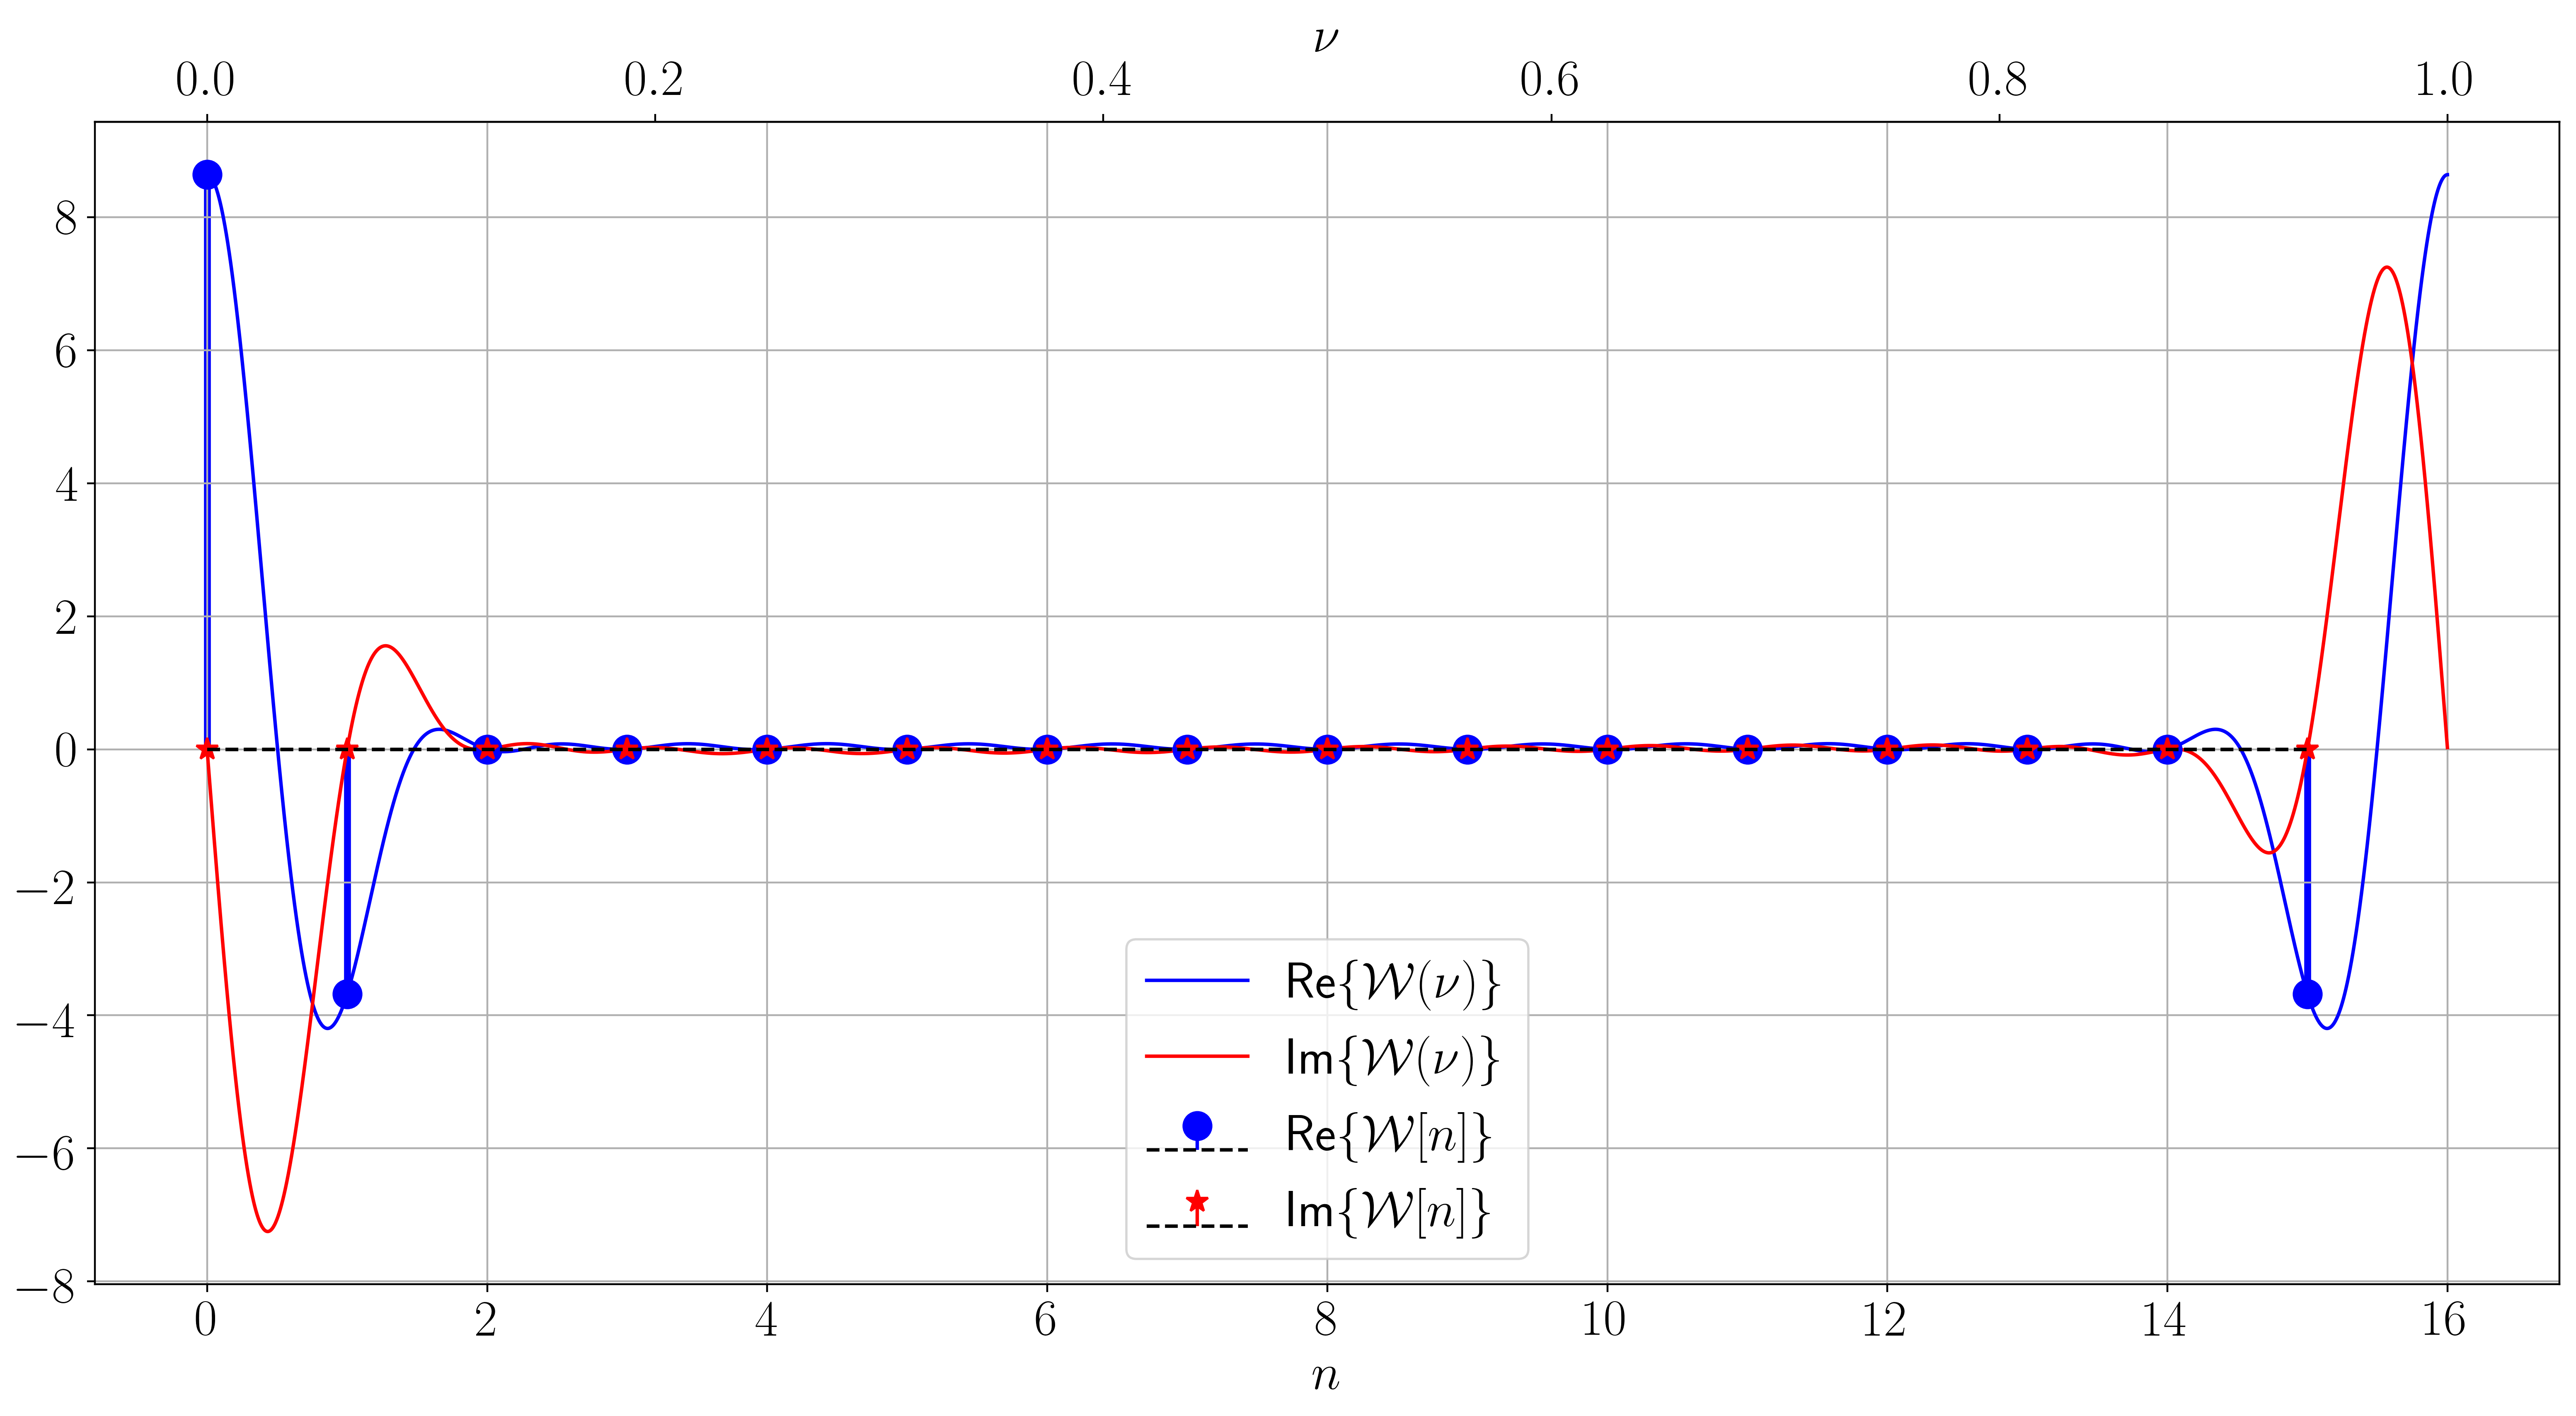
\includegraphics[width=1.0\columnwidth]{pics/spring/1/1-1.png}
	%\caption{.}
	\label{fig:1-1}
\end{figure}

\newpage
\section{}
Предположим, что требуется провести ДПФ-анализ сигнала $x[k]$ с использованием окна Ханна
$\s{w}[k]$. Размерность ДПФ, длина окна и длина сигнала равны $N$. Доказать, что для вычисления ДПФ $\Capit{Y}[n]$ сигнала $x[k]\s{w}[k]$ достаточно провести $2N$ сдвигов на один двоичный разряд и $2N$ сложений для коэффициентов ДПФ $\Capit{X}[n]$ последовательности $x[k]$, т.е. показать, что

\begin{equation*}
\Capit{Y}[n] = \dfrac{1}{2}\left(\Capit{X}[n] - \dfrac{1}{2}\left(\Capit{X}[n-1]_N + \Capit{X}[n+1]_N \right)\right).
\end{equation*}

\begin{align*}
y[k] &= x[k]\s{w}[k] = x[k]\left(\dfrac{1}{2} - \dfrac{1}{2}\cos\left(\dfrac{2\pi k}{N}\right)\right) = 
\dfrac{1}{2}x[k]\left(1 - \dfrac{1}{2}\left[\exp\left(+j\frac{2\pi k}{N}\right) + \exp\left(-j\frac{2\pi k}{N}\right)\right]\right) = \\
&= \dfrac{1}{2}\left(x[k] - \dfrac{1}{2}\left[x[k]\exp\left(+j\frac{2\pi k}{N}\right) + x[k]\exp\left(-j\frac{2\pi k}{N}\right)\right]\right).
\end{align*}

Тогда с применением теоремы смещения для ДПФ получим:
\begin{align*}
\Capit{Y}[n] &= \sum \limits_{k=0}^{N-1}y[k]\exp\left(-j \dfrac{2\pi}{N} nk \right) = 
\sum \limits_{k=0}^{N-1}x[k]\left(\dfrac{1}{2} - \dfrac{1}{2}\cos\left(\dfrac{2\pi k}{N}\right)\right)\exp\left(-j \dfrac{2\pi}{N} nk \right) = \\
&= \dfrac{1}{2}\left(\sum \limits_{k=0}^{N-1}x[k]\exp\left(-j \dfrac{2\pi}{N} nk \right) - \dfrac{1}{2}\left[\sum \limits_{k=0}^{N-1} x[k]\exp\left(-j \dfrac{2\pi}{N} (n-1)k \right)
+ \sum \limits_{k=0}^{N-1} x[k]\exp\left(-j \dfrac{2\pi}{N} (n+1)k \right)\right]\right) = \\
&=\dfrac{1}{2}\left(\Capit{X}[n] - \dfrac{1}{2}\Bigg[\Capit{X}[n-1]_N + \Capit{X}[n+1]_N \Bigg]\right).
\end{align*}

\newpage
\section{}
Вычислить ДВПФ и ДПФ последовательности $y[k] = x[k]\s{w}[k]$, где $x[k] = \sin\Big(2\pi\dfrac{3}{16}k\Big)$, a $\s{w}[k]$ --- окно Ханна для ДПФ длины $N = 16$.
Построить графики действительной и мнимой части коэффициентов ДПФ на одном периоде.

\begin{align*}
y[k] &= x[k]\s{w}[k] =  \sin\left(2\pi\dfrac{3}{16}k\right)\cdot \left(\dfrac{1}{2} - \dfrac{1}{2}\cos\left(\dfrac{2\pi k}{N}\right)\right) = -\dfrac{j}{2}\left[\exp\left(+j \dfrac{2\pi}{16} 3k \right) 
- \exp\left(-j \dfrac{2\pi}{16} 3k \right)\right] \times \\ 
&\times \dfrac{1}{2}
\left[1 - \dfrac{1}{2}\left(\exp\left(+j\frac{2\pi k}{N}\right) + \exp\left(-j\frac{2\pi k}{N}\right)\right)\right] = \dfrac{j}{4}\left[-\exp\left(+j \dfrac{2\pi}{16} 3k \right) 
+ \exp\left(-j \dfrac{2\pi}{16} 3k \right)\right] + \\
&+\dfrac{j}{8}\left[
+\exp\left(+j \dfrac{2\pi}{16} 2k \right) 
+ \exp\left(+j \dfrac{2\pi}{16} 4k \right)
- \exp\left(-j \dfrac{2\pi}{16} 4k \right) 
-\exp\left(-j \dfrac{2\pi}{16} 2k \right)\right]. 
\end{align*}

Используя теоремы смещения для ДВПФ и ДПФ, находим, что

\begin{align*}
\Capit{Y}(\nu) &= \sum \limits_{k = 0}^{15} y[k]e^{-j2\pi \nu k} =
\dfrac{j}{4}\left[-\Capit{W}_{\Capit{D}}\left(\nu - \dfrac{3}{16}\right) + \Capit{W}_{\Capit{D}}\left(\nu + \dfrac{3}{16}\right) \right] + \\
&+\dfrac{j}{8}\left[+\Capit{W}_{\Capit{D}}\left(\nu - \dfrac{2}{16}\right) + \Capit{W}_{\Capit{D}}\left(\nu - \dfrac{4}{16}\right) -
\Capit{W}_{\Capit{D}}\left(\nu + \dfrac{4}{16}\right) -
\Capit{W}_{\Capit{D}}\left(\nu + \dfrac{2}{16}\right)\right].%^{\footnotemark}.
\end{align*}
%\footnotetext{$\Capit{W}_{\Capit{D}}(\nu) = \dfrac{\sin (N \pi \nu)}{\sin(\pi \nu)}e^{-j(N-1)\pi \nu}$ -- ДВПФ прямоугольного окна (окна Дирихле) из $N$ отсчётов.}

\begin{equation*}
\Capit{Y}[n] = \begin{cases}
\mp 4j,& \text{ если } n = 16m \pm 3,\; m \in \mathbb{Z}, \\
\pm 2j,& \text{ если } n = 16m \pm 2 \text{ или } n = 16m \pm 4,\; m \in \mathbb{Z}, \\
0,& \text{ иначе}.
\end{cases}
\end{equation*}

\begin{figure}[!h]
	\centering
	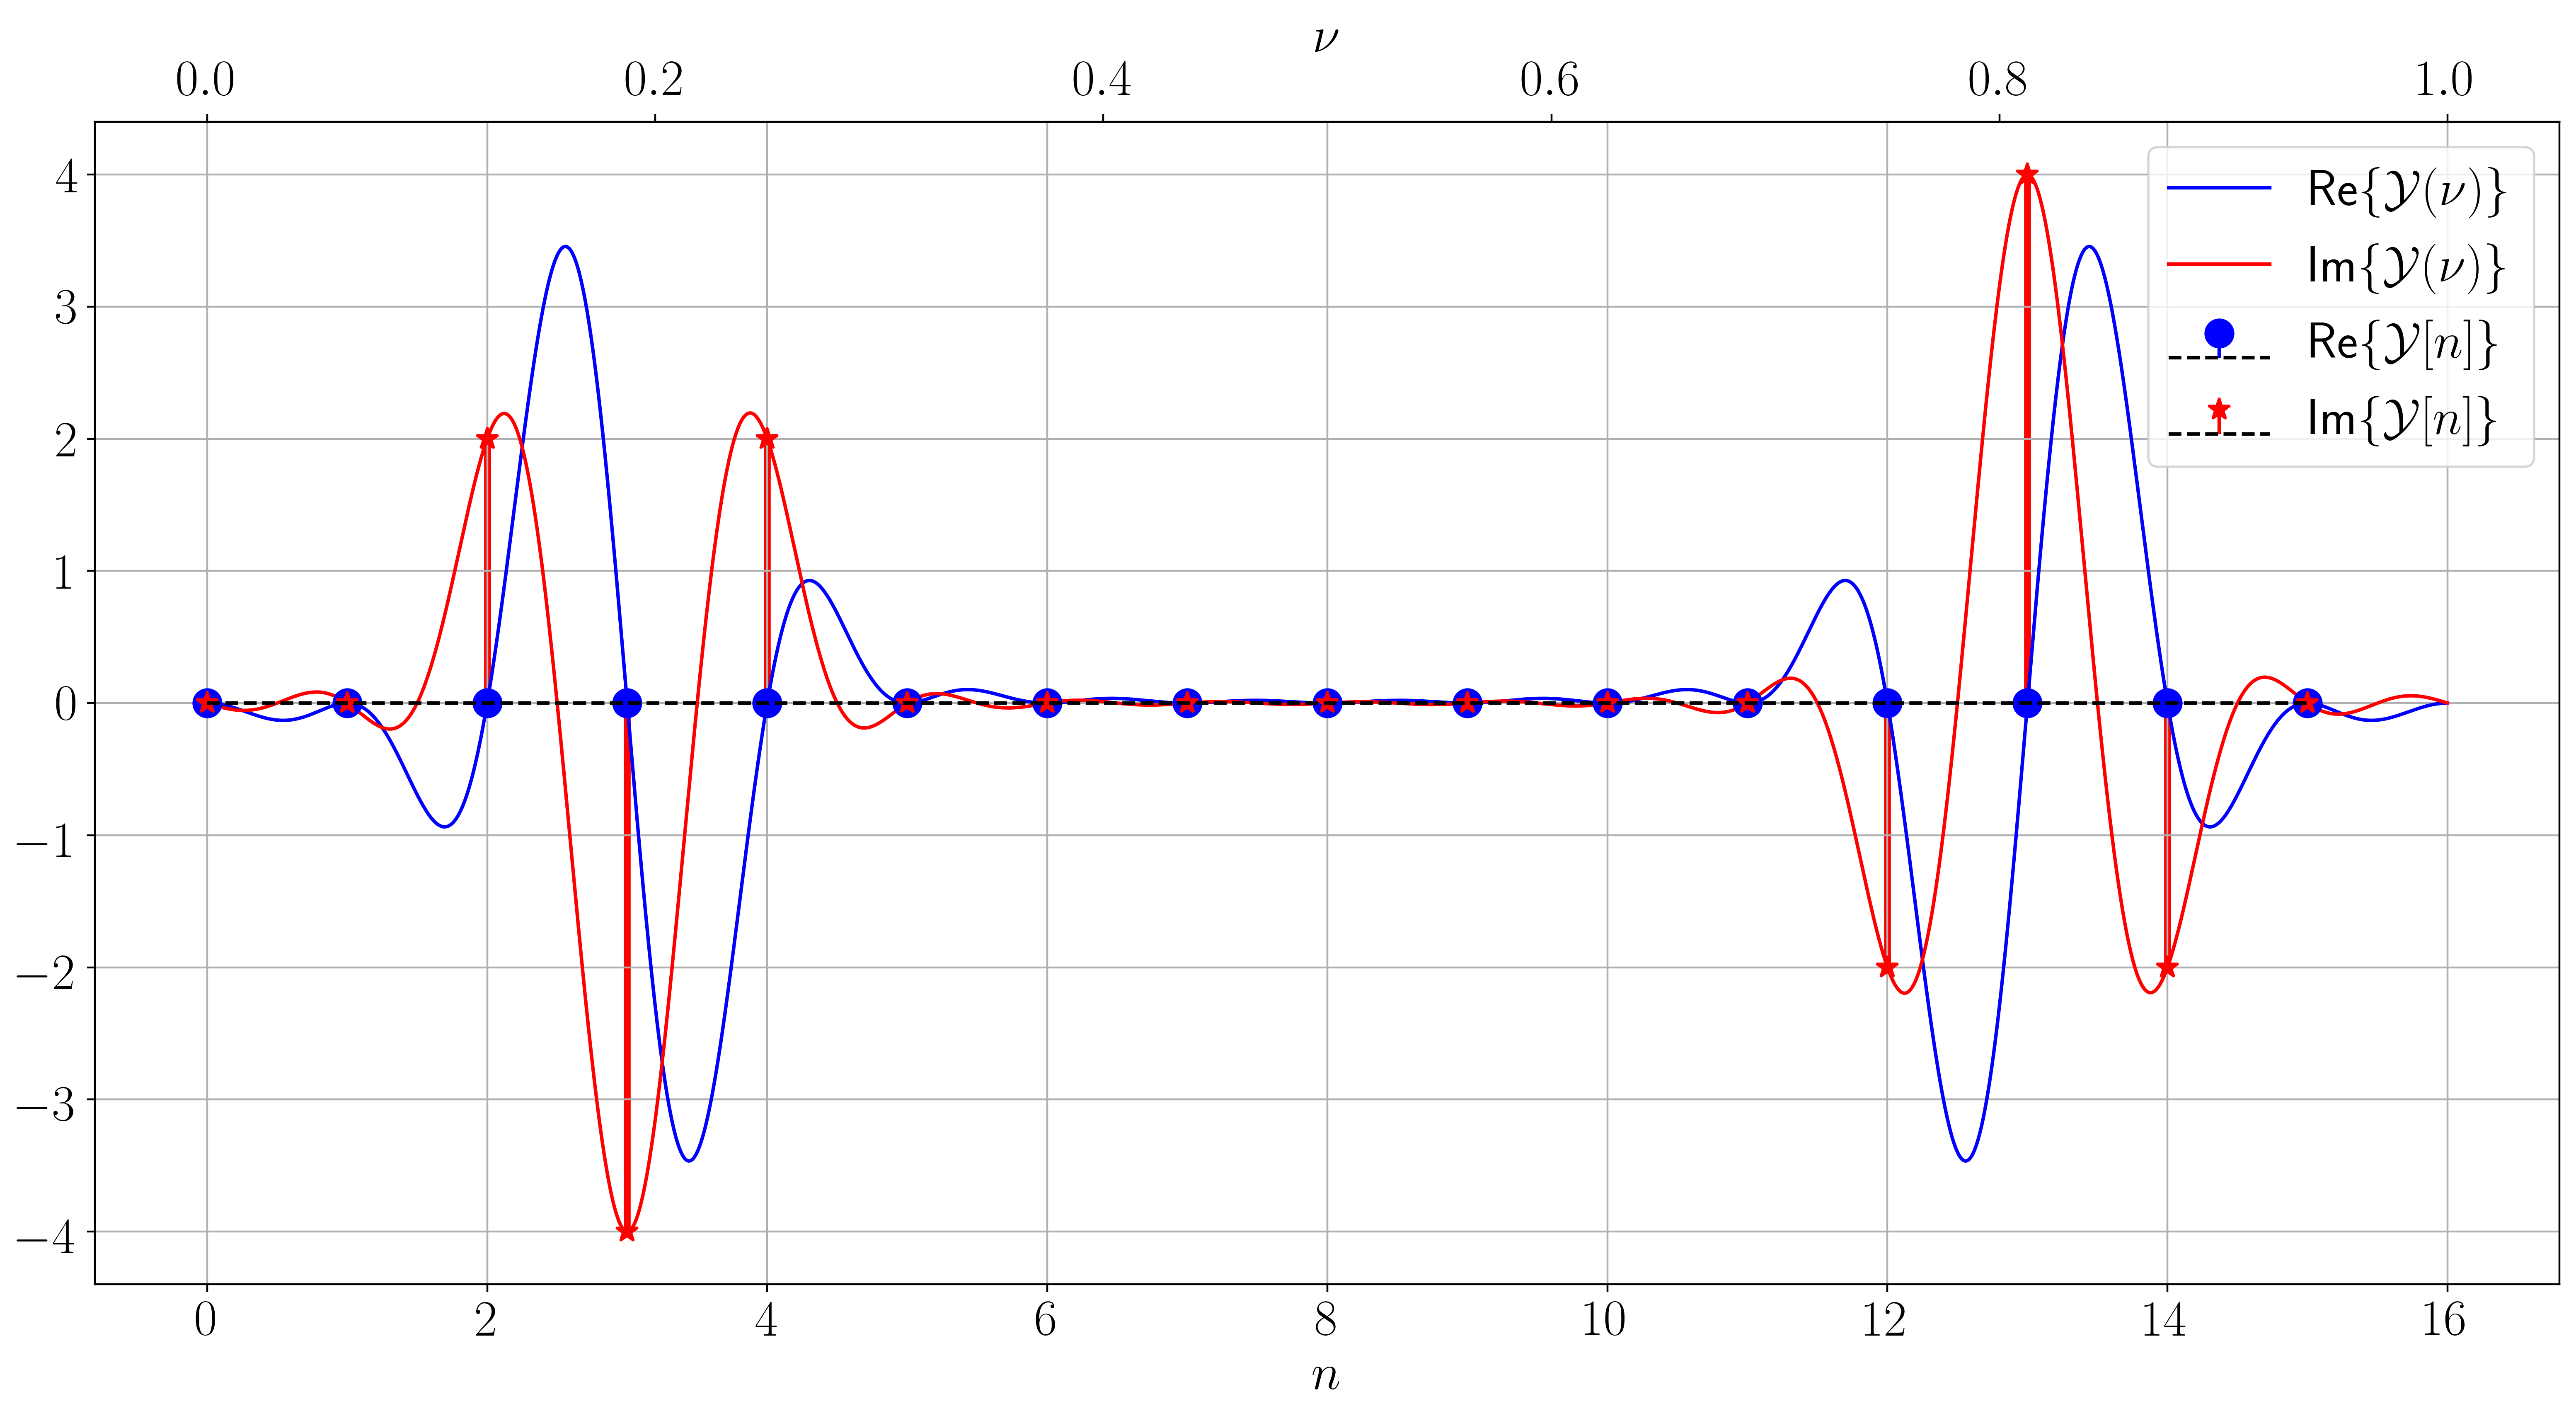
\includegraphics[width=1.\columnwidth]{pics/spring/1/1-3.png}
	%\caption{.}
	\label{fig:1-3}
\end{figure}
